\documentclass[10pt,a4paper]{article}

% Layout
\usepackage[margin=0.8in]{geometry}
\usepackage{fancyhdr}
\usepackage{titlesec}
\usepackage{enumitem}
\usepackage{float}

% Math / Tables
\usepackage{amsmath,amsfonts}
\usepackage{booktabs}

% Graphics / Plots
\usepackage{tikz}
\usepackage{pgfplots}
\pgfplotsset{compat=1.18}

% Fonts / Colors / Links
\usepackage{lmodern}
\renewcommand{\familydefault}{\sfdefault}
\usepackage{xcolor}
\usepackage{hyperref}
\usepackage{tocloft}

% Code listings
\usepackage{listings}

% ---------- Reusable variables ----------
\newcommand{\NoteTitle}{Statistics \& Probability Theory}
\newcommand{\NoteAuthor}{Thomaskutty Reji}

% ---------- Spacing ----------
\setlength{\parskip}{2.5pt}
\setlength{\parindent}{0pt}
\setlength{\headheight}{14pt}
\setlength{\abovedisplayskip}{5pt}
\setlength{\belowdisplayskip}{5pt}
\setlength{\abovedisplayshortskip}{3pt}
\setlength{\belowdisplayshortskip}{3pt}
\setcounter{secnumdepth}{3}

\setlist[itemize]{leftmargin=1.8em,labelwidth=0.8em,labelsep=0.35em,itemsep=2pt,topsep=2pt,parsep=0pt,partopsep=0pt}
\setlist[enumerate]{leftmargin=2.0em,labelsep=0.4em,itemsep=2pt,topsep=2pt,parsep=0pt,partopsep=0pt}

% ---------- Colors ----------
\definecolor{tocblue}{HTML}{0345fc}
\colorlet{accent}{tocblue}

\definecolor{softgreen}{HTML}{E6F4EA}
\definecolor{softyellow}{HTML}{FFF6D6}
\definecolor{softblue}{HTML}{D6E7F8}

\definecolor{codebg}{RGB}{245,245,245}
\definecolor{codeblue}{RGB}{0,70,180}
\definecolor{codecomment}{RGB}{90,90,90}
\definecolor{codestring}{RGB}{160,60,0}

% ---------- Section styles ----------
\titleformat{\section}{\LARGE\color{accent}}{\thesection}{0.8em}{}
\titleformat{\subsection}{\Large\color{accent}}{\thesubsection}{0.8em}{}
\titleformat{\subsubsection}{\large\color{accent}}{\thesubsubsection}{0.8em}{}
\titlespacing*{\section}{0pt}{9pt}{4pt}
\titlespacing*{\subsection}{0pt}{7pt}{3pt}
\titlespacing*{\subsubsection}{0pt}{6pt}{2pt}

% ---------- TOC styles ----------
\renewcommand{\cftsecfont}{\color{tocblue}}
\renewcommand{\cftsubsecfont}{\color{tocblue}}
\renewcommand{\cftsubsubsecfont}{\color{tocblue}}
\renewcommand{\cftsecpagefont}{\color{tocblue}}
\renewcommand{\cftsubsecpagefont}{\color{tocblue}}
\renewcommand{\cftsubsubsecpagefont}{\color{tocblue}}
\setlength{\cftbeforesecskip}{0pt}

% ---------- Header / Footer ----------
\pagestyle{fancy}
\fancyhf{}
\fancyhead[L]{\NoteTitle}
\fancyhead[R]{\textbf{}}
\fancyfoot[L]{\hyperref[toc]{Table of Contents}}
\fancyfoot[R]{\thepage}
\renewcommand{\headrulewidth}{0.4pt}
\renewcommand{\footrulewidth}{0.4pt}

\fancypagestyle{plain}{
  \fancyhf{}
  \fancyhead[L]{\NoteTitle}
  \fancyhead[R]{\textbf{}}
  \fancyfoot[L]{\hyperref[toc]{Table of Contents}}
  \fancyfoot[R]{\thepage}
  \renewcommand{\headrulewidth}{0.4pt}
  \renewcommand{\footrulewidth}{0.4pt}
}

% ---------- Custom commands ----------
\newcommand{\Set}[1]{\left\{#1\right\}}

% ---------- Listings ----------
\lstdefinestyle{github}{
  language=R,
  backgroundcolor=\color{codebg},
  basicstyle=\ttfamily\small,
  keywordstyle=\color{codeblue}\bfseries,
  identifierstyle=\color{black},
  commentstyle=\color{codecomment}\itshape,
  stringstyle=\color{codestring},
  showstringspaces=false,
  frame=single,
  rulecolor=\color{black!20},
  breaklines=true,
  tabsize=4
}

\lstset{
  language=R,
  basicstyle=\ttfamily\small,
  keywordstyle=\color{blue},
  commentstyle=\color{gray},
  stringstyle=\color{orange},
  showstringspaces=false,
  frame=single,
  breaklines=true
}

% ---------- Hyperlinks ----------
\hypersetup{
  colorlinks=true,
  linkcolor=tocblue,
  citecolor=tocblue,
  urlcolor=tocblue
}

\begin{document}

\begin{titlepage}
  \vspace*{0.25\textheight}
  {\LARGE \textcolor{tocblue}{\NoteTitle}}\par
  \author{\NoteAuthor}
  \date{}
\end{titlepage}

\phantomsection
\label{toc}
\tableofcontents
\newpage
	
\section{A/B Testing, A/B/n Testing, and Multivariate Testing}
	
A/B testing is a randomized controlled experiment used to compare two variants of a system to determine which performs better with respect to a predefined metric such as conversion rate or revenue per user. A/B/n testing extends this framework to multiple variants, while multivariate testing decomposes system performance into contributions from multiple factors and their interactions.
	
\subsection{Experimental Design and Group Assignment}

The first step is to define the objective and primary metric (e.g., conversion rate). Users are filtered into the target population (e.g., new users), and then randomly assigned to groups

To ensure balance across important covariates (e.g., geography, device type), stratified randomization is used. The population is divided into strata and randomization is applied within each stratum.

Let strata be indexed by $s$, then:
\[
P(\text{assignment} \mid s) = \text{uniform across variants}
\]

This reduces variance and ensures comparability across groups.
	
\subsection{Sanity Checks}

Before analysis, sanity checks are required:

\begin{itemize}
\item Sample Ratio Mismatch (SRM): verify observed allocation matches expected proportions
\[
\chi^2 = \sum \frac{(O_i - E_i)^2}{E_i}
\]
\item Balance checks: compare distributions of covariates across groups
\item Data quality checks: ensure event logging consistency
\end{itemize}

Failure in these checks invalidates the experiment.
	
\subsection{Statistical Significance Testing}

Let $p_A$ and $p_B$ be conversion rates of control and variant. The null hypothesis is:
\[
H_0: p_A = p_B
\]

A common test is the two-sample z-test:
\[
z = \frac{p_A - p_B}{\sqrt{p(1-p)\left(\frac{1}{n_A} + \frac{1}{n_B}\right)}}
\]
where $p$ is the pooled estimate.
	
\subsection{Numeric Example (A/B Testing)}

\begin{itemize}
\item Variant A: $n_A = 10000$, conversions = 500 $\Rightarrow p_A = 0.05$
\item Variant B: $n_B = 10000$, conversions = 650 $\Rightarrow p_B = 0.065$
\end{itemize}

Pooled estimate:
\[
p = \frac{500 + 650}{20000} = 0.0575
\]

\[
z = \frac{0.065 - 0.05}{\sqrt{0.0575(1-0.0575)\left(\frac{1}{10000}+\frac{1}{10000}\right)}} \approx 4.2
\]

This corresponds to a very small p-value, indicating statistical significance.

Statistical significance indicates the probability of observing data under the null hypothesis. A p-value below a threshold (e.g., 0.05) suggests rejecting $H_0$. However, significance does not imply practical importance.



\subsection{A/B/n Testing}

A/B/n testing compares multiple variants simultaneously. Traffic is split across $k$ variants.

This lab demonstrates an A/B/n testing framework with five variants (A, B, C, D, E), where A serves as the control group and the remaining groups represent different treatment variants. The goal is to evaluate whether changes in design or strategy lead to improvements in user behavior.

The dataset consists of 300 observations, with 60 users assigned to each group. Each observation contains a binary conversion outcome (0 or 1) and a revenue value, where revenue is non-zero only for converted users. This structure reflects a realistic experimental setup commonly used in product and marketing analytics.

The primary metric considered is the conversion rate, defined as the proportion of users who completed the desired action. A secondary metric is revenue, which captures the monetary value generated per user.

\begin{table}[H]
\centering
\begin{tabular}{lrrrr}
\hline
Group & Users & Conversions & Conversion Rate & Avg Revenue \\
\hline
A & 60 & 17 & 0.283 & 29.0 \\
B & 60 & 35 & 0.583 & 58.3 \\
C & 60 & 40 & 0.667 & 65.0 \\
D & 60 & 45 & 0.750 & 75.5 \\
E & 60 & 48 & 0.800 & 84.2 \\
\hline
\end{tabular}
\caption{Summary statistics for each group}
\end{table}


From the summary statistics, the conversion rates across the groups are as follows:
A: 0.283, B: 0.583, C: 0.667, D: 0.750, E: 0.800.  
There is a clear increasing trend from the control group to the final variant, suggesting that each successive treatment improves performance.

To formally test whether these differences are statistically significant, a multi-sample test for equality of proportions was conducted. The null hypothesis states that all groups have equal conversion rates, while the alternative hypothesis states that at least one group differs.

The test produced a p-value of $1.544 \times 10^{-8}$, which is far below the significance level of $\alpha = 0.05$. Therefore, the null hypothesis is rejected, indicating that there is a statistically significant difference in conversion rates across the groups.

\begin{table}[H]
\centering
\begin{tabular}{lcccc}
\hline
& A & B & C & D \\
\hline
B & 0.0174 & - & - & - \\
C & 0.0006 & 1.0000 & - & - \\
D & 0.0000081 & 0.8136 & 1.0000 & - \\
E & 0.00000039 & 0.1769 & 1.0000 & 1.0000 \\
\hline
\end{tabular}
\caption{Pairwise comparison p-values (Bonferroni adjusted)}
\end{table}

To identify which specific groups differ, pairwise comparisons were performed using a Bonferroni correction to control for multiple testing. The results show that:
\begin{itemize}
\item Group A differs significantly from all other groups.
\item Differences among groups B, C, D, and E are mostly not statistically significant after correction.
\item The largest improvements occur when moving from the control (A) to any treatment group.
\end{itemize}

\begin{table}[H]
\centering
\begin{tabular}{lrrrr}
\hline
Comparison & Diff & Lower CI & Upper CI & Adjusted p-value \\
\hline
B - A & 29.27 & 5.14 & 53.39 & 0.0086 \\
C - A & 36.05 & 11.93 & 60.17 & 0.0005 \\
D - A & 46.54 & 22.42 & 70.67 & 0.0000023 \\
E - A & 55.17 & 31.05 & 79.29 & 0.0000000 \\
C - B & 6.78 & -17.34 & 30.91 & 0.9386 \\
D - B & 17.28 & -6.85 & 41.40 & 0.2855 \\
E - B & 25.90 & 1.78 & 50.03 & 0.0284 \\
D - C & 10.49 & -13.63 & 34.62 & 0.7549 \\
E - C & 19.12 & -5.00 & 43.24 & 0.1920 \\
E - D & 8.63 & -15.50 & 32.75 & 0.8635 \\
\hline
\end{tabular}
\caption{Tukey HSD results for revenue comparison}
\end{table}

In addition to conversion, revenue was analyzed as a continuous outcome using one-way ANOVA. The null hypothesis states that the mean revenue is equal across all groups. The ANOVA test yielded a p-value of $9.83 \times 10^{-9}$, indicating strong evidence against the null hypothesis and confirming that revenue differs significantly across groups.

A Tukey post-hoc test was conducted to determine which pairs of groups show significant differences in mean revenue. The results indicate that:
\begin{itemize}
\item All treatment groups (B, C, D, E) generate significantly higher revenue than the control group (A).
\item Differences among higher-performing groups are less pronounced, with only a few pairwise comparisons reaching significance.
\end{itemize}

Overall, both conversion rate and revenue metrics consistently improve from group A to group E. While the global tests confirm statistically significant differences, pairwise comparisons suggest diminishing marginal gains among the top-performing variants.

From a business perspective, group E demonstrates the highest conversion rate and average revenue, making it the strongest candidate for deployment. However, since differences between top variants are not always statistically significant, considerations such as implementation cost, user experience, and robustness should also be taken into account before making a final decision.


\section{Poisson Distribution}

The Poisson distribution is used to model the \textbf{number of events occurring in a fixed interval of time or space}.

\begin{itemize}
 \item Events occur randomly and independently
 \item The average rate of occurrence is constant
 \item We count how many events occur in a fixed interval
\end{itemize}

We denote:
\[
X \sim \text{Poisson}(\lambda), \quad \lambda > 0
\]

\begin{itemize}
 \item $\lambda$ is the \textbf{rate parameter}
 \item Represents the expected number of events in a fixed interval
 \item Example: $\lambda = 5$ means on average 5 events per interval
 \item Larger $\lambda$ $\Rightarrow$ more frequent events
 \item Smaller $\lambda$ $\Rightarrow$ fewer events
\end{itemize}


\subsection{Probability Mass Function (PMF)}

\[
P(X = k) = \frac{\lambda^k e^{-\lambda}}{k!}, \quad k = 0,1,2,\ldots
\]


\subsection{Cumulative Distribution Function (CDF)}

\[
P(X \le k) = \sum_{i=0}^{k} \frac{\lambda^i e^{-\lambda}}{i!}
\]


\subsection{Mean and Variance}

\[
\mathbb{E}[X] = \lambda
\]

\[
\mathrm{Var}(X) = \lambda
\]

\textbf{Interpretation:}
\begin{itemize}
 \item Mean = Variance (key property)
 \item Larger $\lambda$ increases both spread and center
\end{itemize}


\subsection{Derivation of the Mean}

\[
\mathbb{E}[X] = \sum_{k=0}^{\infty} k \cdot \frac{\lambda^k e^{-\lambda}}{k!}
\]

\[
= \lambda
\]


\subsection{Derivation of Variance}

\[
\mathrm{Var}(X) = \mathbb{E}[X^2] - (\mathbb{E}[X])^2
\]

\[
\mathrm{Var}(X) = \lambda
\]


\subsection{Connection to Exponential Distribution}

\begin{itemize}
 \item Poisson models \textbf{counts of events}
 \item Exponential models \textbf{waiting time between events}
 \item If events follow a Poisson process:
 \begin{itemize}
     \item Inter-arrival times are Exponential
     \item Number of events in interval is Poisson
 \end{itemize}
\end{itemize}


\subsection{Shape and Behavior}

\begin{itemize}
 \item For small $\lambda$: right-skewed
 \item For large $\lambda$: approximately normal
 \item Distribution shifts right as $\lambda$ increases
\end{itemize}
	

	\begin{itemize}
	    \item The MLE for $\lambda$ is the sample mean
	    \item Empirical and theoretical probabilities should align well
	    \item Mean and variance should be approximately equal
	    \item Deviations indicate overdispersion or model mismatch
	\end{itemize}
	
	
	\subsection{Model Diagnostics}
	
	\begin{itemize}
	    \item Check if mean $\approx$ variance
	    \item If variance $>$ mean $\Rightarrow$ overdispersion
	    \item If variance $<$ mean $\Rightarrow$ underdispersion
	    \item Consider Negative Binomial if Poisson fails
	\end{itemize}
	
	
	\subsection{Applications}
	
	\begin{itemize}
	    \item Number of calls in a call center per hour
	    \item Number of emails received per day
	    \item Number of accidents at an intersection
	    \item Count of rare events in fixed intervals
	\end{itemize}
	

	\section{Exponential Distribution}
		
		The exponential distribution is used to model the \textbf{waiting time until the occurrence of an event} in a continuous-time setting.
		
		\begin{itemize}
		    \item Events occur randomly over time
		    \item The average rate of occurrence is constant
		    \item We are interested in the time until the first event occurs
		\end{itemize}
		
		We denote:
		\[
		X \sim \text{Exponential}(\lambda), \quad \lambda > 0
		\]
		
		\begin{itemize}
		    \item $\lambda$ is called the \textbf{rate parameter}
		    \item Think of $\lambda$ as Expected number of events per unit time
		    \item For $\lambda = 0.2$, the process generates about $0.2$ events per unit time, i.e., on average about $2$ events in $10$ time units.
		    \item The rate is time-independent: events occur randomly over time, but with a stable average rate that does not change with time.
		    \item Larger $\lambda$ $\Rightarrow$ faster events $\Rightarrow$ shorter waiting times
		    \item Smaller $\lambda$ $\Rightarrow$ slower events $\Rightarrow$ longer waiting times
		\end{itemize}
		
		
		
		\subsection{Probability Density Function (PDF)}
		
		The probability density function is given by:
		
		\[
		f(x) = \lambda e^{-\lambda x}, \quad x \ge 0
		\]
		
		
		\textbf{Properties:}
		\begin{itemize}
		    \item $f(x) \ge 0$
		    \item $\int_0^{\infty} f(x)\,dx = 1$
		\end{itemize}
		
		\textbf{Interpretation:}  
		The density $f(x)$ describes how likely the event is to occur around time $x$.
		
		
		
		\subsection{Cumulative Distribution Function (CDF)}
		
		
		\[
		F(x) = P(X \le x) = \int_0^x \lambda e^{-\lambda t} dt
		\]
		
		\[
		F(x) = 1 - e^{-\lambda x}
		\]
		
		\textbf{Interpretation:}  
		The probability that the event has occurred by time $x$.
		
		
		
		\subsection{Survival Function}
		
		\[
		S(x) = P(X > x) = 1 - F(x) = e^{-\lambda x}
		\]
		
		\textbf{Interpretation:}  
		The probability that the event has not yet occurred by time $x$.
		
		
		\subsection{Mean and Variance}
		
		\[
		\mathbb{E}[X] = \frac{1}{\lambda}
		\]
		
		\[
		\mathrm{Var}(X) = \frac{1}{\lambda^2}
		\]
		
		\textbf{Interpretation:}
		\begin{itemize}
		    \item The expected waiting time is inversely proportional to the rate
		    \item Higher rate $\Rightarrow$ smaller mean waiting time
		\end{itemize}
		
		
		\subsection{Derivation of the Mean}
		
		\[
		\mathbb{E}[X] = \int_0^{\infty} x \lambda e^{-\lambda x} dx
		\]
		
		Using integration by parts:
		
		Let:
		\[
		u = x, \quad dv = \lambda e^{-\lambda x} dx
		\]
		
		\[
		du = dx, \quad v = -e^{-\lambda x}
		\]
		
		Then:
		\[
		\mathbb{E}[X] = \left[-x e^{-\lambda x}\right]_0^\infty + \int_0^\infty e^{-\lambda x} dx
		\]
		
		\[
		= 0 + \frac{1}{\lambda}
		\]
		
		\[
		\Rightarrow \mathbb{E}[X] = \frac{1}{\lambda}
		\]
		
		\subsection{Derivation of Variance}
		
		The variance is given by:
		\[
		\mathrm{Var}(X) = \mathbb{E}[X^2] - (\mathbb{E}[X])^2
		\]
		
		First compute:
		\[
		\mathbb{E}[X^2] = \int_0^\infty x^2 \lambda e^{-\lambda x} dx
		\]
		
		Using integration by parts:
		\[
		\mathbb{E}[X^2] = 2 \int_0^\infty x e^{-\lambda x} dx
		\]
		
		\[
		= \frac{2}{\lambda^2}
		\]
		
		Thus:
		\[
		\mathrm{Var}(X) = \frac{2}{\lambda^2} - \frac{1}{\lambda^2}
		= \frac{1}{\lambda^2}
		\]
		
		\subsection{Memoryless Property}
		
		The exponential distribution satisfies the memoryless property:
		
		
		\[
		P(X > s + t \mid X > s) = P(X > t)
		\]
		
		
		\textbf{Interpretation:}
		\begin{itemize}
		    \item The future waiting time does not depend on how much time has already passed
		    \item The process has no memory
		\end{itemize}
		
		\textbf{Proof:}
		
		\[
		P(X > s+t \mid X > s) = \frac{P(X > s+t)}{P(X > s)}
		\]
		
		\[
		= \frac{e^{-\lambda (s+t)}}{e^{-\lambda s}} = e^{-\lambda t}
		\]
		
		\[
		= P(X > t)
		\]
		
		\subsection{Shape and Behavior}
		
		\begin{itemize}
		    \item The density function is highest at $x=0$ and decreases exponentially
		    \item The distribution is right-skewed
		    \item Most events occur early, with a long tail for larger values
		    \item Higher $\lambda$ implies shorter expected waiting time:
		    \[
		    \mathbb{E}[T] = \frac{1}{\lambda}
		    \]
		    
		    \item For a fixed time $t$, a higher $\lambda$ increases the probability that the event occurs early:
		    \[
		    P(T \le t) = 1 - e^{-\lambda t}
		    \]
		    
		    \item Thus, larger $\lambda$ leads to faster occurrence of events and higher probability of occurrence within a given time interval.
		\end{itemize}
		


\section{Survival Analysis}
Survival analysis deals with modeling the time until an event of interest occurs. Common examples include time to death, failure of a machine, or customer churn.

A key feature of survival data is the presence of censoring, where the event of interest is not observed for all individuals within the study period.

\subsection{Survival Function}
The survival function is defined as:
\[
S(t) = P(T > t)
\]


Interpretation: The probability that the event has not occurred by time $t$.
	
	
\subsection{Hazard Function}

The hazard function is defined as:

\[
h(t) = \lim_{\Delta t \to 0} \frac{P(t \leq T < t + \Delta t \mid T \geq t)}{\Delta t}
\]

Interpretation: The instantaneous rate at which events occur at time $t$, given survival up to time $t$.


\subsection{Kaplan--Meier Estimator}

The Kaplan--Meier estimator is a non-parametric estimator of the survival function:

\[
\hat{S}(t) = \prod_{t_i \leq t} \left(1 - \frac{d_i}{n_i}\right)
\]

where:
\begin{itemize}
 \item $n_i$ = number at risk just before time $t_i$
 \item $d_i$ = number of events at time $t_i$
 \item KM → estimates survival directly.
 \item KM is not a “first step in modeling" — it’s a separate non-parametric estimator
\end{itemize}


\begin{center}
\begin{tabular}{c|cccccccccccc}
\hline
Time  & 2 & 3 & 6 & 6 & 7 & 10 & 15 & 15 & 16 & 27 & 30 & 32 \\
\hline
Event & 1 & 0 & 1 & 1 & 1 & 0 & 1 & 1 & 1 & 1 & 1 & 1 \\
\hline
\end{tabular}
\end{center}

Note: $1$ indicates event occurred, $0$ indicates right censoring.

\begin{center}
\begin{tabular}{ccccccc}
\hline
Time & $n_i$ & $d_i$ & $\hat{S}(t)$ & Std. Err & Lower 95\% CI & Upper 95\% CI \\
\hline
2  & 12 & 1 & 0.917 & 0.0798 & 0.7729 & 1.000 \\
6  & 10 & 2 & 0.733 & 0.1324 & 0.5148 & 1.000 \\
7  & 8  & 1 & 0.642 & 0.1441 & 0.4132 & 0.996 \\
15 & 6  & 2 & 0.428 & 0.1565 & 0.2089 & 0.876 \\
16 & 4  & 1 & 0.321 & 0.1495 & 0.1287 & 0.800 \\
27 & 3  & 1 & 0.214 & 0.1325 & 0.0635 & 0.720 \\
30 & 2  & 1 & 0.107 & 0.1005 & 0.0169 & 0.675 \\
32 & 1  & 1 & 0.000 & NaN    & NA     & NA \\
\hline
\end{tabular}
\end{center}


At time $t = 2$:
\[
\hat{S}(2) = 1 \times \left(1 - \frac{1}{12}\right) = \frac{11}{12} = 0.917
\]

At time $t = 6$:
\[
\hat{S}(6) = 0.917 \times \left(1 - \frac{2}{10}\right)
= 0.917 \times 0.8 = 0.733
\]

At time $t = 7$:
\[
\hat{S}(7) = 0.733 \times \left(1 - \frac{1}{8}\right)
= 0.733 \times 0.875 = 0.642
\]


The Kaplan--Meier estimator is also known as the product-limit estimator:

\[
\hat{S}(t) = \prod_{t_i \le t} \left(1 - \frac{d_i}{n_i}\right)
\]

This arises from decomposing the survival probability into conditional probabilities:


\[
P(T > t) = \prod_{t_i \le t} P(T > t_i \mid T \ge t_i)
\]

Each term represents the probability of surviving past time $t_i$ given survival up to that point

Thus, the overall survival probability is obtained by multiplying these conditional survival probabilities across all observed event times.


Censored observations:
\begin{itemize}
 \item Contribute to the risk set ($n_i$)
 \item Do not contribute to event count ($d_i$)
\end{itemize}

Example:
\begin{itemize}
 \item At time 3 and 10, observations are censored
 \item They reduce future risk sets but do not affect survival probability directly
\end{itemize}


\begin{itemize}
 \item The survival curve is a step function
 \item Drops occur only at event times
 \item Larger drops indicate higher event rates
 \item Increasing uncertainty over time due to fewer individuals at risk
\end{itemize}


\begin{figure}[H]
\centering
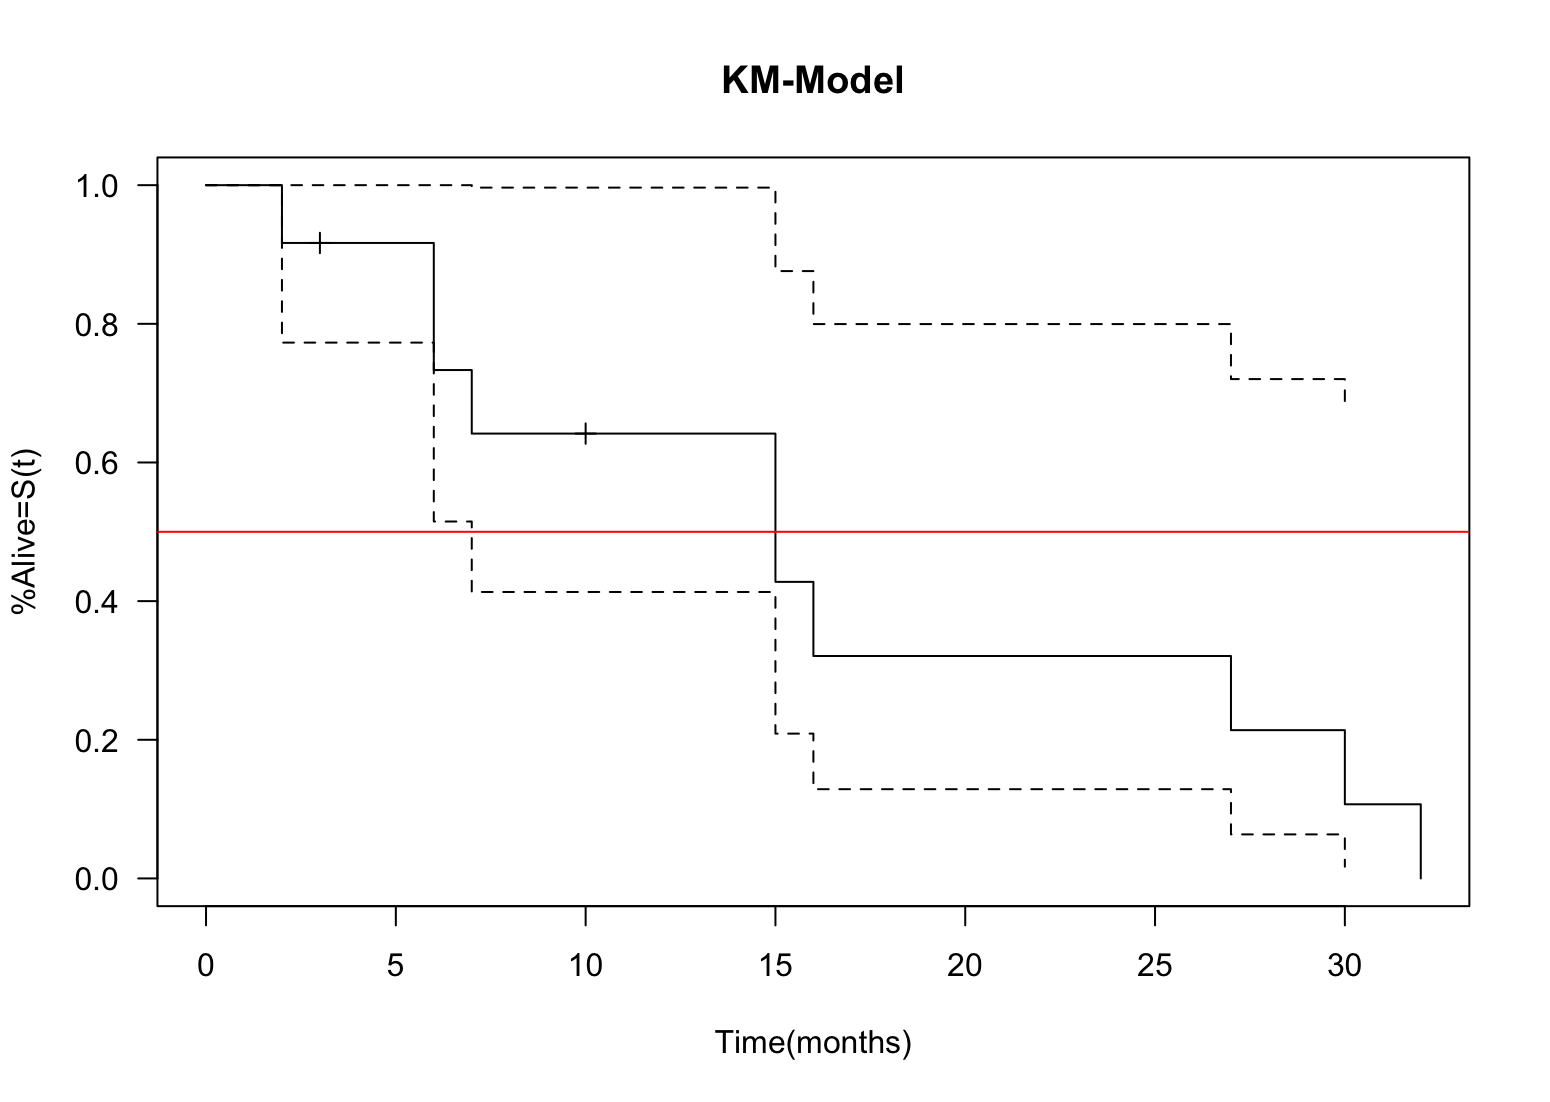
\includegraphics[width=0.7\textwidth]{images/km-model-basic.png}
\caption{Kaplan--Meier survival curve}
\end{figure}


The median survival time is defined as the smallest time $t$ such that:
\[
\hat{S}(t) \leq 0.5
\]

In this dataset, the survival probability drops below 0.5 at $t = 15$, hence the median survival time is 15.

Interpretation: Approximately 50\% of the individuals experience the event by time 15.

\subsection{Survival Analysis (Kaplan-Meier Estimator) with Two Treatment Groups}



We consider a dataset of 20 patients undergoing treatment for a disease. Patients are divided into two groups:

\begin{itemize}
 \item Treatment A (standard)
 \item Treatment B (new treatment)
\end{itemize}

For each patient, we observe:
\begin{itemize}
 \item Time to event (in months)
 \item Event indicator (1 = death, 0 = censored)
 \item Treatment group
\end{itemize}



\begin{center}
\resizebox{\textwidth}{!}{
\begin{tabular}{c|cccccccccccccccccccc}
\hline
& 1 & 2 & 3 & 4 & 5 & 6 & 7 & 8 & 9 & 10 
& 11 & 12 & 13 & 14 & 15 & 16 & 17 & 18 & 19 & 20 \\
\hline
Time      & 2 & 3 & 6 & 6 & 7 & 10 & 15 & 15 & 16 & 27 
       & 4 & 5 & 8 & 9 & 12 & 14 & 18 & 20 & 22 & 25 \\
Status    & 1 & 0 & 1 & 1 & 1 & 0 & 1 & 1 & 1 & 1 
       & 1 & 1 & 0 & 1 & 0 & 1 & 0 & 1 & 1 & 0 \\
Treatment & A & A & A & A & A & A & A & A & A & A 
       & B & B & B & B & B & B & B & B & B & B \\
Age       & 65 & 70 & 72 & 68 & 66 & 74 & 69 & 71 & 67 & 73 
       & 60 & 62 & 59 & 63 & 61 & 64 & 58 & 66 & 65 & 67 \\
\hline
\end{tabular}
}
\end{center}

\begin{center}
\begin{tabular}{ccccccc}
\hline
Time & $n_i$ & $d_i$ & $\hat{S}(t)$ & Std.Err & Lower CI & Upper CI \\
\hline
2  & 10 & 1 & 0.900 & 0.0949 & 0.7320 & 1.000 \\
6  & 8  & 2 & 0.675 & 0.1551 & 0.4303 & 1.000 \\
7  & 6  & 1 & 0.563 & 0.1651 & 0.3165 & 1.000 \\
15 & 4  & 2 & 0.281 & 0.1631 & 0.0903 & 0.876 \\
16 & 2  & 1 & 0.141 & 0.1286 & 0.0234 & 0.844 \\
27 & 1  & 1 & 0.000 & NaN    & NA     & NA \\
\hline
\end{tabular}
\end{center}


\begin{center}
\begin{tabular}{ccccccc}
\hline
Time & $n_i$ & $d_i$ & $\hat{S}(t)$ & Std.Err & Lower CI & Upper CI \\
\hline
4  & 10 & 1 & 0.900 & 0.0949 & 0.7320 & 1.000 \\
5  & 9  & 1 & 0.800 & 0.1265 & 0.5868 & 1.000 \\
9  & 7  & 1 & 0.686 & 0.1515 & 0.4447 & 1.000 \\
14 & 5  & 1 & 0.549 & 0.1724 & 0.2963 & 1.000 \\
20 & 3  & 1 & 0.366 & 0.1884 & 0.1332 & 1.000 \\
22 & 2  & 1 & 0.183 & 0.1600 & 0.0329 & 1.000 \\
\hline
\end{tabular}
\end{center}


\begin{figure}[H]
\centering
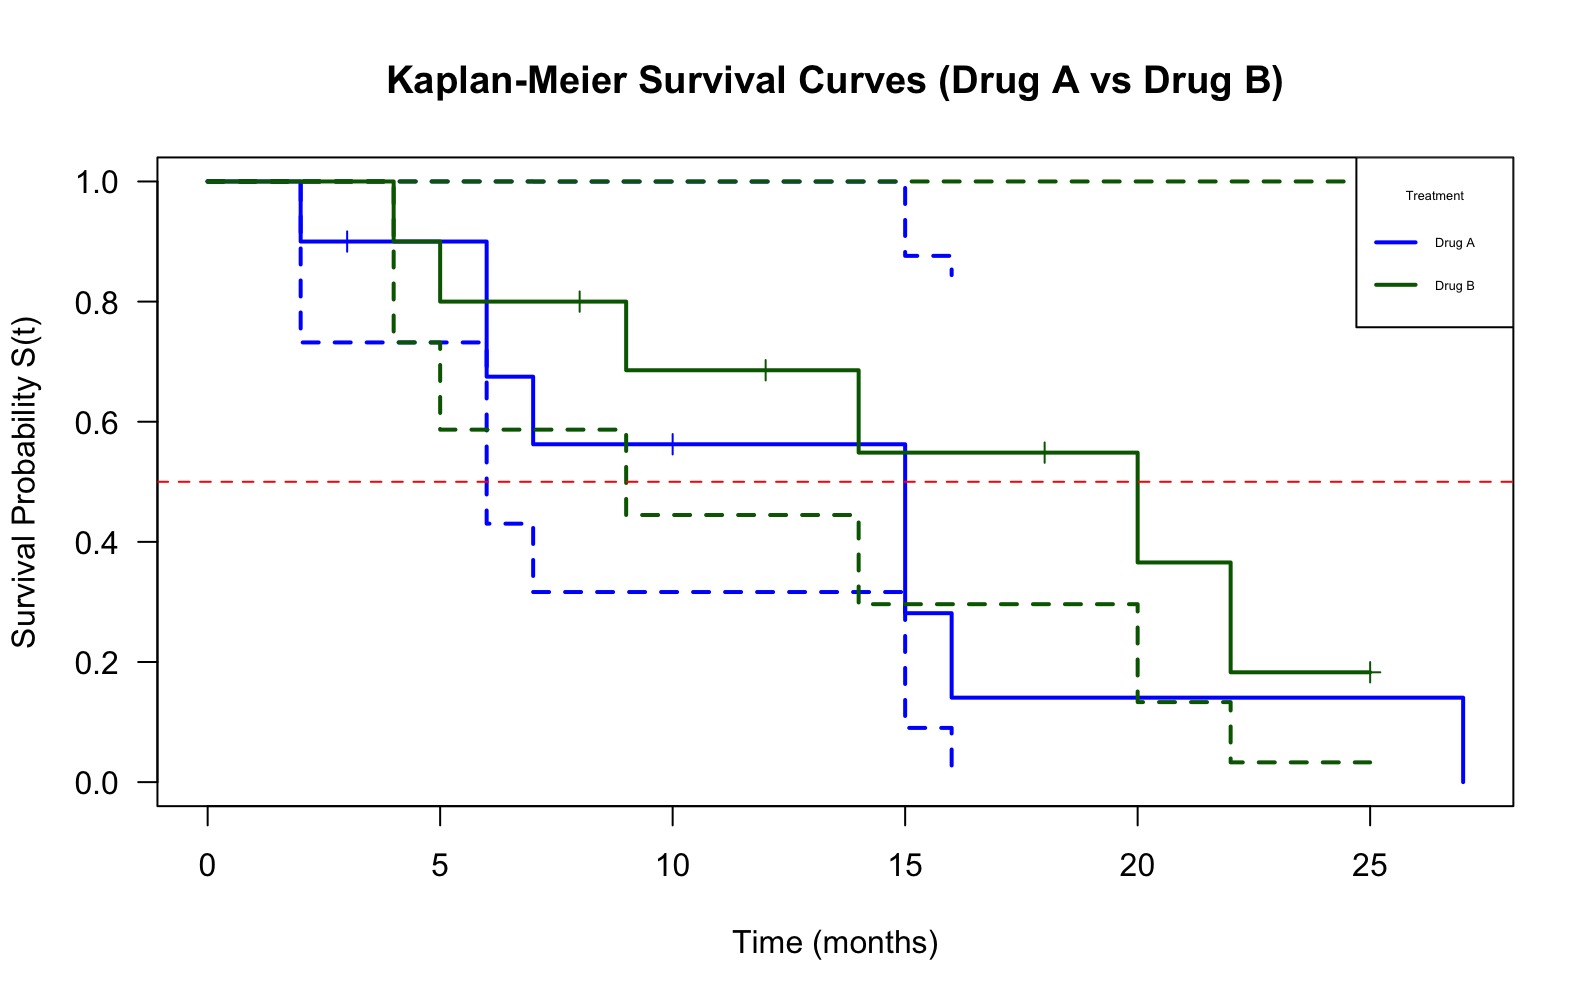
\includegraphics[width=0.6\textwidth]{images/Survival_analysis_groups-kme.png}
\caption{Kaplan--Meier Survival Curves for Treatment A and B}
\end{figure}


\begin{itemize}
 \item Treatment B generally shows higher survival probabilities at later times.
 \item Treatment A experiences more rapid decline in survival.
 \item The difference between curves is visible but not very large.
\end{itemize}



\textbf{Median Survival}
\begin{itemize}
 \item Treatment A reaches survival below 0.5 earlier.
 \item Treatment B maintains survival above 0.5 for longer.
 \item Interpretation: Patients receiving Treatment B tend to survive longer.
\end{itemize}


\textbf{Statistical Significance (Log-Rank Test)}
\begin{itemize}
 \item Null hypothesis: Survival curves are identical.
 \item Test statistic: $\chi^2 = 0.6$
 \item p-value = 0.4
 \item Since $p = 0.4 > 0.05$, we fail to reject the null hypothesis.
 \item There is \textbf{no statistically significant difference} between the two treatment groups.
\end{itemize}



%------------------------------------------------------------------------

\subsection{Exponential Model (Intro to Regression Models for Survival)}

The exponential model assumes a constant hazard rate:
\[
h(t) = \lambda, \quad \lambda > 0
\]


 \begin{align*}
f(t) &= \lambda e^{-\lambda t} 
&& \text{(PDF: density at time } t\text{)} \\[6pt]
F(t) &= 1 - e^{-\lambda t} 
&& \text{(CDF: } P(T \le t)\text{, probability event occurs by time } t\text{)} \\[6pt]
S(t) &= e^{-\lambda t} 
&& \text{(Survival: } P(T > t)\text{, probability of surviving beyond } t\text{)}
\end{align*}



The key assumption of the exponential model is:The hazard is constant over time.

\begin{itemize}
\item The risk of failure in the next instant does not depend on how long the individual has survived
\item This is known as the \textbf{memoryless property}
\end{itemize}

To allow different individuals to have different risks, we model:

\begin{align*}
h(t \mid X) = \lambda(X) \\ 
h(t \mid X) = \exp(X\beta)
\end{align*}



\begin{itemize}
\item Ensures $h(t \mid X) \ge 0$
\item Provides a linear structure on the log scale:
\[
\log h(t \mid X) = X\beta
\]
\item Coefficients are interpretable:
\begin{itemize}
\item $e^{\beta_j}$ represents the multiplicative effect on the hazard
\end{itemize}
\end{itemize}


Each individual follows an exponential distribution:
\[
T_i \sim \text{Exponential}(\lambda_i), \quad \lambda_i = \exp(X_i \beta)
\]

\begin{itemize}
\item Same functional form across individuals
\item Different hazard levels depending on covariates
\end{itemize}


 \[
S(t \mid X) = \exp\left(-e^{X\beta} \cdot t\right)
\]



\begin{itemize}
\item Larger $X\beta$ leads to faster decay of survival
\item Smaller $X\beta$ leads to slower decay
\end{itemize}


\paragraph{Likelihood Derivation for Exponential Regression Model}

Let $T_i$ denote the survival time for individual $i$, and let $\delta_i \in \{0,1\}$ be the event indicator, where $\delta_i = 1$ if the event is observed and $\delta_i = 0$ if the observation is right-censored. Let $t_i$ be the observed time.

For an exponential model with rate $\lambda_i$, the density and survival functions are:
\[
f(t_i \mid \lambda_i) = \lambda_i e^{-\lambda_i t_i}, \qquad
S(t_i \mid \lambda_i) = P(T_i > t_i) = e^{-\lambda_i t_i}.
\]

The likelihood contribution depends on what is observed:

- If $\delta_i = 1$, the exact event time is observed, so the contribution is $f(t_i)$.
- If $\delta_i = 0$, the event time is not observed; we only know $T_i > t_i$, so the contribution is $S(t_i)$.

Thus, the likelihood contribution for observation $i$ can be written as:
\[
L_i = f(t_i)^{\delta_i} S(t_i)^{1-\delta_i}.
\]

Substituting the exponential forms:
\[
L_i = \left(\lambda_i e^{-\lambda_i t_i}\right)^{\delta_i} \cdot \left(e^{-\lambda_i t_i}\right)^{1-\delta_i}.
\]

Simplifying:
\[
L_i = \lambda_i^{\delta_i} e^{-\lambda_i t_i \delta_i} \cdot e^{-\lambda_i t_i (1-\delta_i)}
= \lambda_i^{\delta_i} e^{-\lambda_i t_i}.
\]

Hence, the full likelihood is:
\[
L = \prod_{i=1}^n \lambda_i^{\delta_i} e^{-\lambda_i t_i}.
\]

Taking logs:
\[
\ell = \sum_{i=1}^n \left( \delta_i \log \lambda_i - \lambda_i t_i \right).
\]

Now assume a log-linear model for the hazard:
\[
\lambda_i = \exp(x_i^\top \beta).
\]

\[
\ell = \sum_{i=1}^n \left( \delta_i x_i^\top \beta - t_i \exp(x_i^\top \beta) \right).
\]

Define:
\[
\mu_i = t_i \lambda_i = t_i \exp(x_i^\top \beta),
\]
which can be interpreted as the expected number of events over exposure time $t_i$ under a constant hazard $\lambda_i$.

Then:
\[
\ell = \sum_{i=1}^n \left( \delta_i \log \lambda_i - \mu_i \right)
= \sum_{i=1}^n \left[ \delta_i (\log \mu_i - \log t_i) - \mu_i \right].
\]
\[
\ell = \sum_{i=1}^n \left( \delta_i \log \mu_i - \mu_i \right) - \sum_{i=1}^n \delta_i \log t_i.
\]

The second term does not depend on $\beta$, hence the likelihood is equivalent (up to an additive constant) to:
\[
\ell \propto \sum_{i=1}^n \left( \delta_i \log \mu_i - \mu_i \right),
\]

which is the log-likelihood of a Poisson model with mean $\mu_i = t_i \exp(x_i^\top \beta)$ and observed counts $\delta_i$, with $\log t_i$ acting as an offset.


Coefficients are first estimated on the AFT scale and then converted to hazard ratios using
\[
\mathrm{HR}=e^{-\beta}.
\]
This is why we report both model coefficients (for inference) and hazard ratios (for practical risk comparison).

\begin{table}[H]
\centering
\caption{Coefficient Table with Hazard Ratios and 95\% CI}
\begin{tabular}{lrrrrrrr}
\toprule
Variable & Value & Std.\ Error & z & p & H Ratio & lower(95\%) &upper(95\%) \\
\midrule
(Intercept)       & -1.6538 & 2.2450 & -0.737 & 0.4613 & 5.227 & 0.064 & 425.858 \\
age               &  0.0636 & 0.0394 &  1.617 & 0.1058 & 0.938 & 0.869 & 1.014 \\
treatmentNewDrug  &  1.2172 & 0.5921 &  2.056 & 0.0398 & 0.296 & 0.093 & 0.945 \\
\bottomrule
\end{tabular}
\end{table}


Interpretation (compact):
\begin{itemize}
\item Age: HR $=0.938$ per 1-year increase; direction suggests lower hazard with age in this sample, but $p=0.11$ is not strong at 5\%.
\item Treatment: HR $=0.296$ for NewDrug vs Standard; hazard is lower for NewDrug, with statistical support ($p=0.04$).
\item Global model test ($p=0.026$): predictors jointly improve fit over intercept-only.
\end{itemize}

Predictions are generated to convert coefficients into patient-level risk quantities (hazard and probabilities at clinically useful horizons).


\begin{table}[H]
\centering
\caption{Predicted risk summary}
\begin{tabular}{lccccc}
\toprule
Age & Treatment & Hazard/month & Survival (6m) & Event Prob. (12m) & Median Survival (months) \\
\midrule
50 & Standard & 0.2168 & 0.2723 & 0.9259 & 3.20 \\
60 & NewDrug  & 0.0340 & 0.8156 & 0.3348 & 20.41 \\
65 & NewDrug  & 0.0247 & 0.8622 & 0.2566 & 28.05 \\
\bottomrule
\end{tabular}
\end{table}

So, coefficients tell us \emph{direction/significance}, hazard ratios tell us \emph{relative risk}, and predictions tell us \emph{absolute risk and expected survival for specific patients}.

\section{Probability \& Likelihood}

\subsection{Probability}
\textbf{Definition:} Probability quantifies the likelihood of a particular outcome given a known model or set of parameters. It answers:
\begin{quote}
\emph{``What is the chance of observing this outcome, assuming the model and its parameters are true?''}
\end{quote}

\textbf{Perspective:} Forward-looking. Start with model parameters and compute the probability of data.

\textbf{Mathematical Formulation:}
\[
P(X \mid \theta)
\]
where:
\begin{itemize}
\item $X$ : Observed data or event
\item $\theta$ : Parameters of the model
\end{itemize}

\textbf{Example:}  
For a fair coin with $P(\text{Head}) = 0.5$, the probability of observing 3 heads in 5 flips is computed using the binomial distribution.


\subsection{Likelihood}
\textbf{Definition:} Likelihood measures how plausible a set of model parameters is given the observed data. It answers:
\begin{quote}
\emph{``How well does this set of parameters explain the observed data?''}
\end{quote}

\textbf{Perspective:} Backward-looking. Start with observed data and evaluate different parameter values.

\textbf{Mathematical Formulation:}
\[
L(\theta \mid X) = P(X \mid \theta)
\]
Conceptually, $X$ is fixed and $\theta$ varies.

\textbf{Example:}  
Given 3 heads in 5 flips, likelihood helps determine the value of $\theta = P(\text{Head})$ that best explains the observed data.


\subsection{Key Differences}
\begin{center}
\begin{tabular}{|l|l|l|}
\hline
\textbf{Aspect} & \textbf{Probability} & \textbf{Likelihood} \\
\hline
Purpose & Predict future data/events & Estimate model parameters \\
\hline
Input & Model parameters ($\theta$) & Observed data ($X$) \\
\hline
Output & Chance of observing data & Plausibility of parameters \\
\hline
Role in Inference & Forward problems & Parameter estimation (MLE) \\
\hline
Fixed vs Variable & $\theta$ fixed, $X$ varies & $X$ fixed, $\theta$ varies \\
\hline
\end{tabular}
\end{center}


\subsection{Maximum Likelihood Estimation (MLE)}

\textbf{Concept:}  
MLE aims to find parameter values that maximize the likelihood of the observed data.

\textbf{Likelihood Function:}
\[
L(\theta \mid X) = \prod_{i=1}^{n} f(X_i \mid \theta)
\]

\textbf{MLE Estimator:}
\[
\hat{\theta} = \arg\max_{\theta} L(\theta \mid X)
\]


\subsection{Log-Likelihood}
To simplify computation, take logarithms:
\[
\ell(\theta \mid X) = \log L(\theta \mid X) = \sum_{i=1}^{n} \log f(X_i \mid \theta)
\]

Maximizing $\ell(\theta \mid X)$ is equivalent to maximizing $L(\theta \mid X)$.


\subsection{Steps in MLE}
\begin{enumerate}
    \item Specify the probabilistic model
    \item Write the likelihood function
    \item Compute the log-likelihood
    \item Differentiate and solve:
    \[
    \frac{\partial \ell(\theta \mid X)}{\partial \theta} = 0
    \]
\end{enumerate}


\subsection{Example: Normal Distribution}

Assume $X_1, \ldots, X_n \sim \mathcal{N}(\mu, \sigma^2)$.

\textbf{Log-Likelihood:}
\[
\ell(\mu, \sigma^2 \mid X) =
-\frac{n}{2}\log(2\pi)
-\frac{n}{2}\log(\sigma^2)
-\frac{1}{2\sigma^2} \sum_{i=1}^{n}(X_i - \mu)^2
\]

\textbf{MLE Estimates:}
\[
\hat{\mu} = \frac{1}{n}\sum_{i=1}^{n} X_i, \quad
\hat{\sigma}^2 = \frac{1}{n}\sum_{i=1}^{n}(X_i - \hat{\mu})^2
\]


\subsection{Properties of MLE}
\begin{itemize}
    \item Consistency: $\hat{\theta} \to \theta$ as $n \to \infty$
    \item Asymptotic Normality
    \item Efficiency under regularity conditions
\end{itemize}


\subsection{Challenges}
\begin{itemize}
    \item Non-convex optimization landscapes
    \item Lack of closed-form solutions
    \item Overfitting in high-dimensional settings
\end{itemize}


\subsection{Applications}
MLE underpins:
\begin{itemize}
    \item Logistic Regression
    \item Gaussian Mixture Models
    \item Hidden Markov Models
    \item Neural Networks (via negative log-likelihood)
\end{itemize}


\subsection{Further Directions}
\begin{itemize}
    \item Maximum A Posteriori (MAP) Estimation
    \item Numerical Optimization (Newton-Raphson, Gradient Ascent, EM)
    \item Bayesian Inference
\end{itemize}


\end{document}
